\documentclass[12pt]{article}

\usepackage[margin=0.8 in]{geometry}
\usepackage{amsmath}
\usepackage{amssymb}
\usepackage{macros}
\usepackage{mathtools}
\usepackage{enumerate}
\usepackage{verbatim}
\usepackage{amsthm}

\title{}
%\content{}



\let \proj \undefined
\renewcommand{\tr}{ \mathrm{tr}}
\DeclareMathOperator{\SU}{SU}
\DeclareMathOperator{\proj}{proj}
\newcommand{\sS}{\mathscr{S}}
\DeclareMathOperator{\comp}{comp}
\newcommand{\A}{\mathcal{A}}
\renewcommand{\D}{\mathcal{D}}
\renewcommand{\e}{\epsilon}
\newcommand{\Are}{\A_{r,\e}}
\newcommand{\Kre}{K_{r,\e}}
\newcommand{\Dre}{\D_{r,\e}}
\newcommand{\rt}{\tilde{r}}
\newcommand{\et}{\tilde{\e}}
\newtheorem{definition}{Definition}
\newenvironment{solution}
  {\begin{proof}[Solution]}
  {\end{proof}}
\newtheorem{example}{Example}
\newtheorem{exercise}{Exercise}
\usepackage{hyperref}
\newcommand{\vr}{\mathbf{r}}
\newcommand{\vF}{\mathbf{F}}

\newtheorem{theorem}{Theorem}

\begin{document}
\section{Section 15.1-2. Double integrals/Iterated Integrals}
(The \textit{Mathematica} graphics for this section are made by my colleague Tim Mesikepp. You can find a link to his webpage here: \url{https://sites.math.washington.edu/~mesiket/})


Goals for the day: \begin{enumerate}
\item Remember the pictures 
\item Be able to evaluate double 
integrals over rectangles using Fubini's theorem.
\end{enumerate}

\textbf{Question: } In an introductory course on integration (like Math 125), what was the main motivation for defining the integral of a function of one variable?\\
\textbf{Answer}: To compute the area under the graph of the function.
 
 By analogy, when we have a function $ f(x,,y)$ of two variables, defined over a rectangle $$R=[a,b]\times [c,d]=\{(x,y):a\leq x\leq b, c\leq x\leq d \}$$ the main motivation for defining the integral is to calculate the volume of the solid lying under the graph of $f$ and above the domain where it is defined (later in the course we will see some other applications of double integrals as well.).
 
\vspace {.1 in}

Let's see how we define a double integral. Suppose $f(x,y)$ is continuous, non-negative and defined on the rectangle $R$ and we would like to find the volume of the solid lying under the graph of $f$ and above the rectangle $R$. If we had a very special case of a constant function, then we'd know what to do! The solid lying above the rectangle and below the graph of $f$ would be a cuboid, so the volume would be

$$Volume=f(x^*)\times Area(R)=f(x^*)\times(b-a)\times(d-c),$$
where $x^*$ is any point in the rectangle (it doesn't matter which one we choose, since $f$ is constant!).



\begin{figure}
\centering
\parbox{5cm}{
\includegraphics[width=5cm]{untitled.jpg}
\caption{The graph of a constant function}
\label{fig:2figsA}}
\qquad
\begin{minipage}{5cm}
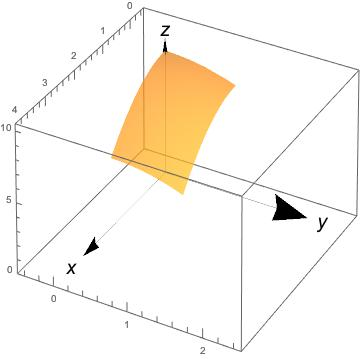
\includegraphics[width=5cm]{graph.jpg}
\caption{The graph of the function $f(x,y)=x^2-y^2$}
\label{fig:2figsB}
\end{minipage}
\end{figure}



Now in general things aren't that nice: $f$ need not be constant. However, if the rectangle is sufficiently small, then we can assume that $f$ is almost constant in it. 

So, we may split the interval $[a,b]$ into $m$ subintervals of length $\Delta x:=\frac{b-a}{m}$ and split $[c,d]$ into $n$ subintervals of length $\Delta y:=\frac{d-c}{n}$, where $m$, $n$ are large integers. In this way $R$ is split into $m\times n$ subrectangles of area $\Delta A := \Delta x\times \Delta y$. Also, consider a number $x_i^*$ in the $i-$th subinterval of $[a,b]$ and $y_j^*$ in the $j-$th subinterval of $[c,d]$.

Now if we assume that $m$, $n$ are large enough, we can assume that $f$ is almost constant in each of the subrectangles, and so the volume under its graph is almost $$\sum_{i=1}^m\sum_{j=1}^n f(x_i^*,y_j^*)\Delta A.$$

This is called  \textbf{Riemann Sum}. By making $m$ and $n$ larger and larger, the approximation improves.

\begin{figure}
\centering
\parbox{5cm}{
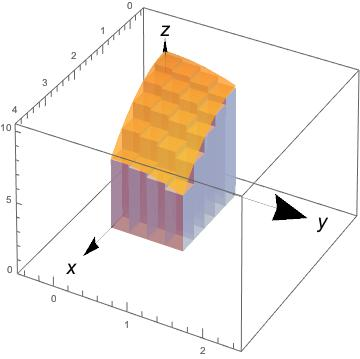
\includegraphics[width=5cm]{boxes54.jpg}
\caption{Approximation of the volume of the solid under our function for $m=5$, $n=4$}
}
\qquad
\begin{minipage}{5cm}
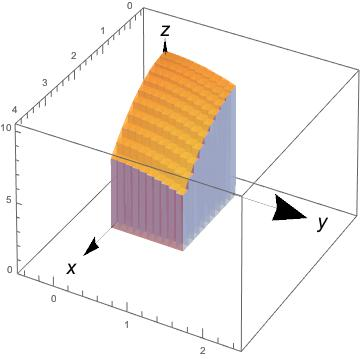
\includegraphics[width=5cm]{boxes1010.jpg}
\caption{Approximation of the volume of the solid under our function for $m=10$, $n=10$}

\end{minipage}
\end{figure}






 We end up defining:


\begin{definition}

If $f(x,y)$ is a continuous non-negative function defined on a rectangle $R$ as before, we let $$\iint_R f(x,y) dA:=\lim_{m\to \infty}\lim_{n\to\infty} \sum_{i=1}^m\sum_{j=1}^n f(x_i^*,y_j^*)\Delta A.$$
If $f$ is non-positive, we define $$\iint_R f(x,y) dA:=-\iint_R (-f)(x,y) dA.$$
\end{definition}


\textbf{Remark:} In this class we will define various types of integrals. However, the idea behind all of those definitions is the same: when we have to integrate a function over a domain, we split the domain in small enough pieces where the function can be assumed to be well behaved.
\vspace{.1 in}

Now this definition might be intuitive (at least to some extent), but it is almost completely useless for practical purposes! Trying to evaluate the integral of anything remotely complicated would be a nightmare. 

So here's another (very informal) approach towards finding the volume of the solid under the graph of $f$ and above the rectangle $R$: Let's slice the solid with the plane $x=const.$. Then, the area of the slice would be the area under the curve $f(x,y)$, for $y\in [c,d]$, which can be computed by $$A(x)=\int_c^d f(x,y)dy,$$ as we know from Math 125. Now to find the volume, we could "add the areas of infinitely many infinitely thin slices", that is, integrate, and find that $$Volume = \int_c^d A(x)dx=\int_a^b\int_c^d f(x,y)dydx.$$

\begin{figure}
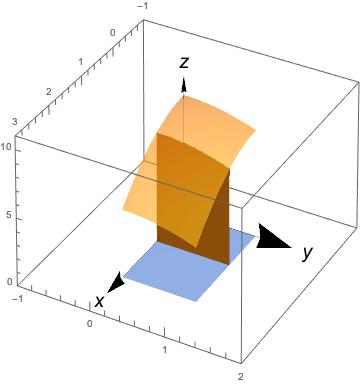
\includegraphics[scale=.4]{fubini.jpg}
\caption{A visualization of Fubini's theorem}
\end{figure}


This results to the following very important (and very hard to prove rigorously) theorem by Fubini:
\begin{theorem}{(Fubini)}
If $f(x,y)$ is continuous, defined on the rectangle $R=[a,b]\times [c,d]=\{(x,y):a\leq x\leq b, c\leq x\leq d \},$ then $$\iint_Rf(x,y) dA=\int_c^d(\int_a^b  f(x,y)dx)dy= \int_a^b(\int_c^df(x,y)dy)dx$$
\end{theorem}
Remarks:
\begin{enumerate}
\item We have no assumption on $f$ being non-negative!
\item Here we are integrating over rectangles and we have the freedom to perform the integration in any order we like with the appropriate bounds. However later, once we'll be dealing with more complicated domains than rectangles, we'd have to be a bit more careful.

\end{enumerate}


Let's see an example:
\begin{example}
(15.2/Problem 30): Find the volume of the solid in the first octant, bounded by $z=16-x^2$, $y=5$.
\end{example}
\begin{solution}
Let's draw a picture:

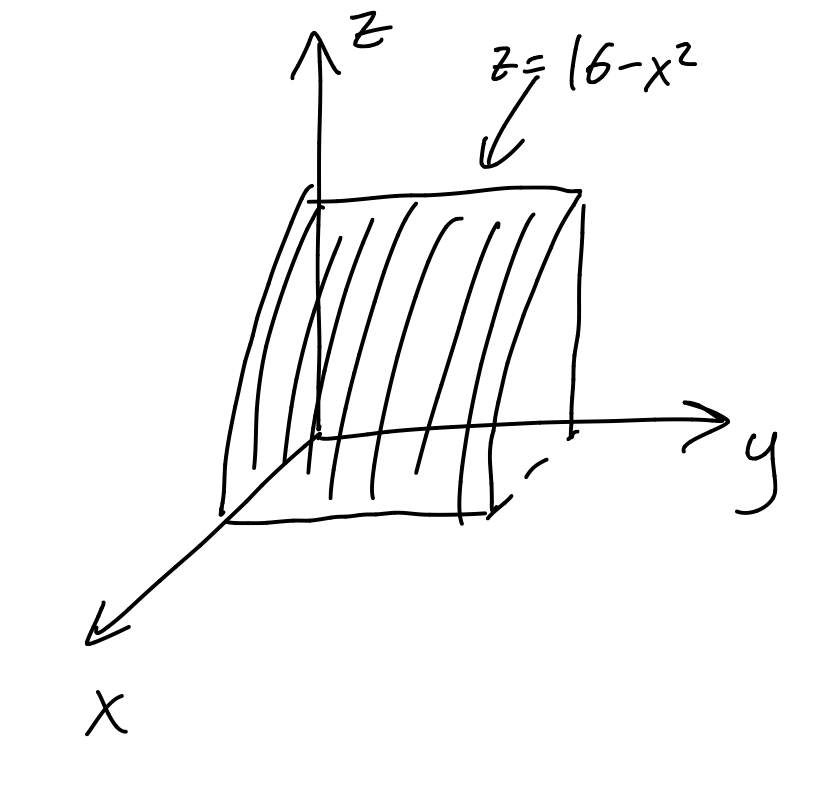
\includegraphics[scale=.1]{picture.jpeg}

Since we're in the first octant, we know that $x\geq 0$, $y\geq 0$ and $ z\geq 0$. We're also bounded by the plane $y=5$, so $y\leq 5$. Looking at the picture, we see that the bound for $x$ is determined by the intersection of $z=16-x^2$ and the $xy$ plane, so $z=0\implies 16-x^2=0\implies x=\pm 4$, and we keep $x=4$ because we live in the first octant. Therefore, by Fubini's theorem,\begin{align*}Volume=\int_0^5\int_0^416-x^2 dx dy=&\int_0^5\big[16x-x^3/3\big]_0^4 dy\\
 =&\int_0^5 64-64/3dy\\
 =&640/3.\end{align*}
\end{solution}
\end{document}

